\documentclass[conference,letterpaper,10pt]{IEEEtran}
\IEEEoverridecommandlockouts

\usepackage{cite}
\usepackage{amsmath,amssymb}
\usepackage{graphicx}
\usepackage{booktabs}
\usepackage{array}
\usepackage{tabularx}
\usepackage{xcolor}
\usepackage{tikz}
\usetikzlibrary{positioning,arrows.meta,shapes.misc}
\usepackage{url}
\usepackage[hidelinks]{hyperref}

% All numbers quoted in the text come from results/ through this generated file.
% Generated by build_report_assets.py from results/. Do not edit by hand.
\newif\ifdebias\debiastrue
\newcommand{\nTrain}{29{,}879}
\newcommand{\nVal}{3{,}736}
\newcommand{\nTest}{3{,}735}
\newcommand{\nTotal}{37{,}350}
\newcommand{\nHateTotal}{10{,}619}
\newcommand{\hatePct}{28.4}
\newcommand{\nHateTest}{1{,}062}
\newcommand{\bodyShamingTrain}{92}
\newcommand{\bodyShamingTest}{14}
\newcommand{\religiousTest}{18}
\newcommand{\originTest}{23}
\newcommand{\personalOffenseTrain}{5{,}752}
\newcommand{\consistencyViolations}{0}
\newcommand{\urlRows}{3}
\newcommand{\dupTrain}{8}
\newcommand{\testInTrain}{1}
\newcommand{\medianWords}{7}
\newcommand{\pNinetyFiveWords}{27}
\newcommand{\paperHateTotal}{10{,}282}
\newcommand{\paperBodyShamingTrain}{68}
\newcommand{\tokPNinetyNine}{108}
\newcommand{\maxLen}{128}
\newcommand{\truncPct}{0.6}
\newcommand{\trainMinutes}{18.4}
\newcommand{\bestEpoch}{4}
\newcommand{\binThr}{0.58}
\newcommand{\nParams}{278}
\newcommand{\binF}{76.23}
\newcommand{\binMacroAcc}{75.99}
\newcommand{\binAcc}{80.83}
\newcommand{\hateP}{66.80}
\newcommand{\hateR}{64.78}
\newcommand{\binFHalf}{75.50}
\newcommand{\mlFall}{19.53}
\newcommand{\subsetAll}{72.37}
\newcommand{\hammAll}{4.34}
\newcommand{\mlFhate}{28.89}
\newcommand{\microFhate}{57.66}
\newcommand{\subsetHate}{31.45}
\newcommand{\hammHate}{11.03}
\newcommand{\mlFhateHalf}{30.08}
\newcommand{\catPO}{56.2}
\newcommand{\catPOHate}{67.1}
\newcommand{\catAV}{46.6}
\newcommand{\catAVHate}{50.1}
\newcommand{\catPol}{35.8}
\newcommand{\catPolHate}{50.7}
\newcommand{\catGen}{10.3}
\newcommand{\catGenHate}{23.5}
\newcommand{\catMisc}{7.3}
\newcommand{\catMiscHate}{8.2}
\newcommand{\catRel}{0.0}
\newcommand{\catRelHate}{19.0}
\newcommand{\catOri}{0.0}
\newcommand{\catOriHate}{0.0}
\newcommand{\catBody}{0.0}
\newcommand{\catBodyHate}{12.5}
\newcommand{\nFN}{374}
\newcommand{\pctFN}{35.2}
\newcommand{\nFP}{342}
\newcommand{\pctFP}{12.8}
\newcommand{\blXlmrBin}{77.35}
\newcommand{\blXlmrAcc}{81.37}
\newcommand{\blXlmrMl}{29.29}
\newcommand{\blBanglaBertBin}{76.50}
\newcommand{\blBestBin}{77.36}
\newcommand{\blBestBinModel}{TB-mBERT}
\newcommand{\blBestMl}{39.53}
\newcommand{\blBestMlModel}{GPT 4o + Few-shot}
\newcommand{\blBestMlFt}{30.17}
\newcommand{\blBestMlFtModel}{TB-BERT}
\newcommand{\gapBin}{1.12}
\newcommand{\gapMl}{0.40}
\newcommand{\topThreeOverlap}{0.71}
\newcommand{\ratSample}{100}
\newcommand{\ratA}{93}
\newcommand{\ratB}{57}
\newcommand{\ratBoth}{55}
\newcommand{\ratWords}{551}
\newcommand{\kappaVal}{0.559}
\newcommand{\rawAgree}{78.4}
\newcommand{\faithN}{91}
\newcommand{\plNA}{91}
\newcommand{\auprcLimeA}{0.805}
\newcommand{\tokFLimeA}{0.683}
\newcommand{\iouFLimeA}{0.527}
\newcommand{\auprcShapA}{0.808}
\newcommand{\tokFShapA}{0.715}
\newcommand{\iouFShapA}{0.604}
\newcommand{\auprcRandomA}{0.627}
\newcommand{\tokFRandomA}{0.518}
\newcommand{\iouFRandomA}{0.352}
\newcommand{\plNB}{55}
\newcommand{\auprcLimeB}{0.777}
\newcommand{\tokFLimeB}{0.658}
\newcommand{\iouFLimeB}{0.545}
\newcommand{\auprcShapB}{0.777}
\newcommand{\tokFShapB}{0.690}
\newcommand{\iouFShapB}{0.600}
\newcommand{\auprcRandomB}{0.567}
\newcommand{\tokFRandomB}{0.466}
\newcommand{\iouFRandomB}{0.327}
\newcommand{\compHuman}{0.41}
\newcommand{\suffHuman}{-0.02}
\newcommand{\compLime}{0.47}
\newcommand{\suffLime}{-0.13}
\newcommand{\compShap}{0.48}
\newcommand{\suffShap}{-0.13}
\newcommand{\compRandom}{0.16}
\newcommand{\suffRandom}{0.18}
\newcommand{\biasNA}{69}
\newcommand{\biasNB}{31}
\newcommand{\biasFlagA}{18}
\newcommand{\biasFlagB}{1}
\newcommand{\biasFprA}{26.1}
\newcommand{\biasFprB}{3.2}
\newcommand{\biasMeanPA}{0.33}
\newcommand{\biasMeanPB}{0.12}
\newcommand{\biasShapTop}{55.1}
\newcommand{\biasNWords}{30}
\newcommand{\hrKuttar}{94}
\newcommand{\hrKukur}{82}
\newcommand{\hrBaccha}{77}
\newcommand{\hrPagol}{59}
\newcommand{\hrHindu}{30}
\newcommand{\hrBnp}{24}
\newcommand{\trainHatePct}{28.4}
\newcommand{\debNWords}{99}
\newcommand{\debMinCount}{20}
\newcommand{\debMinRate}{60}
\newcommand{\debNRepeated}{1{,}307}
\newcommand{\debTrainRows}{33{,}800}
\newcommand{\debBinF}{75.46}
\newcommand{\debBinAcc}{74.43}
\newcommand{\debMlF}{22.05}
\newcommand{\debFprA}{18.8}
\newcommand{\debFprB}{0.0}
\newcommand{\debTestOldWith}{74.8}
\newcommand{\debTestNewWith}{33.8}
\newcommand{\debTestOldWithout}{9.1}
\newcommand{\debTestNewWithout}{9.2}
\newcommand{\debTestNWith}{151}
\newcommand{\debTestNWithout}{2{,}522}
\newcommand{\debBestEpoch}{2}
\newcommand{\debThr}{0.48}
\newcommand{\debBinDrop}{0.77}
\newcommand{\debMlDrop}{6.84}
\newcommand{\debSubsetHate}{13.18}


\newcommand{\yes}{\checkmark}
\newcommand{\no}{--}

\begin{document}

\title{Explainable Multi-Label Hate Speech Detection in Transliterated Bangla Using Transformer Models}

\author{
\IEEEauthorblockN{Md. Israfil Hossain\IEEEauthorrefmark{1},
Md. Biplob\IEEEauthorrefmark{1},
Diab Alam\IEEEauthorrefmark{1},
Ifta Faisal\IEEEauthorrefmark{1},
Md. Faiyaz Ullah Adin\IEEEauthorrefmark{1}}
\IEEEauthorblockA{\IEEEauthorrefmark{1}Department of Computer Science and Engineering, United International University, Dhaka, Bangladesh\\
Course: CSE 4889 Machine Learning\\
% TODO: add student IDs, e.g. Md. Israfil Hossain (ID: 0112XXXXXX)
Student IDs: [to be added]}
}

\maketitle

\begin{abstract}
Bangladeshi social media users often write Bangla in Latin script, mixing it with English. Hate speech detectors trained on standard-script text handle this poorly, and the few systems built for transliterated Bangla give no reason for their decisions. We fine-tune a dual-head XLM-RoBERTa model on the BanTH dataset that predicts whether a comment is hateful and which of eight target categories apply. On the official test split the model reaches a binary macro-F1 of \binF\% and a multi-label macro-F1 of \mlFhate\% on hate comments, on par with the strongest published fine-tuned baselines but not above them. Our main contribution is the evaluation of the explanations. We explain predictions with LIME and SHAP and compare them with word-level rationales that two annotators marked on \ratSample{} test comments (Cohen's $\kappa$ = \kappaVal). SHAP explanations match human rationales clearly better than a random baseline (token F1 \tokFShapA{} vs.\ \tokFRandomA) and are faithful to the model: deleting the top-ranked words lowers the predicted hate probability by \compShap{} on average, against \compRandom{} for random words. A keyword-bias test on harmless sentences shows that \biasFprA\% of sentences containing insult-associated words are wrongly flagged, against \biasFprB\% without such words, and SHAP identifies the triggering word in \biasShapTop\% of cases. Oversampling harmless training comments that contain such words reduces false positives on real non-hate test comments with these words from \debTestOldWith\% to \debTestNewWith\%, at the cost of lower category performance. The system is released as a web application for moderators.
\end{abstract}

\begin{IEEEkeywords}
hate speech detection, transliterated Bangla, multi-label classification, explainable AI, transformers
\end{IEEEkeywords}

% ======================================================================
\section{Introduction}

Online platforms in Bangladesh carry a large volume of user comments written in \emph{transliterated Bangla}, that is, Bangla typed with the Latin alphabet and frequently mixed with English words. The same word can be spelled in many ways (\emph{bhai}, \emph{vai}), and there is no standard orthography. Hate speech in this form is common in comment sections of news and political videos, yet most Bangla hate speech resources use the Bangla script~\cite{romim2022bdshs,hasan2026banglamultihate}.

Content moderators, non-governmental organisations that monitor online harm, and researchers need more than a hate/non-hate label. They need to know \emph{which group} a comment targets, and they need a \emph{reason} they can check before acting on a prediction. The BanTH dataset~\cite{haider2025banth} addressed the first need by providing multi-label target annotations for transliterated Bangla, but the models evaluated on it produce no explanations. Rationale-annotated benchmarks such as HateXplain~\cite{mathew2021hatexplain} for English and HateBRXplain~\cite{salles2025hatebrxplain} for Brazilian Portuguese have shown that explanations must be evaluated against human judgement, because post-hoc explanations can look sensible without reflecting what the model used.

\textbf{Gap.} To our knowledge, no prior work provides a rationale-grounded, faithfulness-evaluated explainable multi-label hate speech system for transliterated Bangla. Explainable hate speech detection itself has been studied for other languages~\cite{mathew2021hatexplain,salles2025hatebrxplain,yadav2026userbased}; the gap we address is specific to this language setting.

\textbf{Contributions.}
\begin{itemize}
\item A dual-head XLM-RoBERTa~\cite{conneau2020xlmr} classifier for binary and eight-category multi-label detection, trained and tested on the official BanTH splits and compared with the published baselines.
\item A small rationale-annotated test subset (\ratSample{} comments, two annotators) and an evaluation of LIME~\cite{ribeiro2016lime} and SHAP~\cite{lundberg2017shap} for plausibility and faithfulness, following HateXplain and ERASER~\cite{deyoung2020eraser}.
\item A keyword-bias test showing that the model over-flags harmless sentences containing insult-associated words, with explanations that expose the cause, and a data-based mitigation experiment that reduces the bias with a measurable trade-off.
\item A deployed web application that shows the verdict, the target categories and the words behind each decision.
\end{itemize}

% ======================================================================
\section{Related Work}

\subsection{Bangla Hate Speech Datasets}
BD-SHS~\cite{romim2022bdshs} provides more than 50,000 hierarchically annotated Bangla-script comments. BanglaMultiHate~\cite{hasan2026banglamultihate} jointly annotates hate type, severity and target, and compares zero-shot and LoRA-tuned large language models with BanglaBERT. For code-mixed Bangla-English, Fahim et al.~\cite{fahim2025abusive} built a 2,700-comment binary abusive-language dataset with a deep learning ensemble. BanTH~\cite{haider2025banth} is presented as the first multi-label hate speech dataset for transliterated Bangla; it benchmarks fine-tuned encoders, encoders further pre-trained on transliterated text, and GPT prompting strategies, but does not address explanation.

\subsection{Multi-Label Hate Speech in Other Languages}
K-MHaS~\cite{lee2022kmhas} annotates Korean news comments with eight overlapping hate categories, motivated by the intersectionality of hate speech. Its category scheme is close to that of BanTH, but neither work evaluates explanations.

\subsection{Explainable Hate Speech with Rationales}
HateXplain~\cite{mathew2021hatexplain} introduced word-level human rationales for English hate speech and the plausibility and faithfulness metrics we adopt, and showed that strong classifiers do not necessarily produce good explanations. HateBRXplain~\cite{salles2025hatebrxplain} added rationales for Brazilian Portuguese and found that LIME and SHAP explanations were plausible but not faithful for the best models. MFTCXplain~\cite{trager2025mftcxplain} provides span-level rationales and moral categories for multilingual hate speech and finds limited alignment between large language model rationales and human ones, and Ahmed et al.~\cite{ahmed2024bilstmlime} combined a BiLSTM with LIME for English multi-label detection without human evaluation of the explanations.

\subsection{Explainability for Code-Mixed Text}
For Hindi-English misogyny detection, Yadav et al. evaluated SHAP and gradient-based explanations in a user study~\cite{yadav2026userbased} and built a multimodal explainable web application with LIME and SHAP~\cite{yadav2026multimodal}. Both address a single label (misogyny) rather than multi-label hate categories.

Table~\ref{tab:related} summarises these works. None of them combines transliterated Bangla, multi-label targets, human-rationale evaluation and faithfulness testing.

\begin{table*}[t]
\caption{Comparison With Related Work}
\label{tab:related}
\centering
\small
\resizebox{\textwidth}{!}{%
\begin{tabular}{llccccc}
\toprule
Work & Language & Multi-label & Explanations & Human rationales & Faithfulness & Deployed app \\
\midrule
BD-SHS~\cite{romim2022bdshs} & Bangla (script) & hierarchical & \no & \no & \no & \no \\
Fahim et al.~\cite{fahim2025abusive} & Bangla-English & \no & \no & \no & \no & \no \\
BanglaMultiHate~\cite{hasan2026banglamultihate} & Bangla (script) & multi-task & \no & \no & \no & \no \\
BanTH~\cite{haider2025banth} & Transliterated Bangla & \yes & \no & \no & \no & \no \\
K-MHaS~\cite{lee2022kmhas} & Korean & \yes & \no & \no & \no & \no \\
HateXplain~\cite{mathew2021hatexplain} & English & \no{} (3-class) & \yes & \yes & \yes & \no \\
HateBRXplain~\cite{salles2025hatebrxplain} & Portuguese & \no & LIME, SHAP & \yes & \yes & \no \\
MFTCXplain~\cite{trager2025mftcxplain} & Multilingual & \no & LLM & \yes & \no & \no \\
Ahmed et al.~\cite{ahmed2024bilstmlime} & English & \yes{} (3 labels) & LIME & \no & \no & \no \\
Yadav et al.~\cite{yadav2026userbased} & Hindi-English & \no & SHAP, IG & user study & \no & \no \\
Yadav et al.~\cite{yadav2026multimodal} & Hindi-English & \no & LIME, SHAP & \no & \no & \yes \\
\midrule
\textbf{This work} & Transliterated Bangla & \yes & LIME, SHAP & \yes & \yes & \yes \\
\bottomrule
\end{tabular}}
\end{table*}

% ======================================================================
\section{Dataset}
\label{sec:dataset}

\subsection{BanTH}
BanTH~\cite{haider2025banth} contains \nTotal{} YouTube comments in transliterated Bangla, released on Hugging Face~\cite{banth_hf}. Each comment has a binary label and, if hateful, one or more of eight target categories: Political, Religious, Gender, Personal Offense, Abusive/Violence, Origin, Body Shaming and Misc. We use the official splits of \nTrain{}, \nVal{} and \nTest{} comments so that our results are comparable with the published baselines. Hate comments make up \hatePct\% of the data in every split.

Table~\ref{tab:labels} and Fig.~\ref{fig:balance} show the label distribution. The categories are highly imbalanced: Personal Offense has \personalOffenseTrain{} training examples while Body Shaming has only \bodyShamingTrain{}, and the test split contains just \bodyShamingTest{} Body Shaming, \religiousTest{} Religious and \originTest{} Origin comments.

\begin{table}[t]
\caption{Label Distribution in the Official BanTH Splits}
\label{tab:labels}
\centering
\small
\begin{tabular}{lrrrr}
\toprule
Label & Train & Val. & Test & Train (\%) \\
\midrule
Non-hate (Label = 0) & 21{,}384 & 2{,}674 & 2{,}673 & 71.6 \\
Hate (Label = 1) & 8{,}495 & 1{,}062 & 1{,}062 & 28.4 \\
\midrule
Political & 978 & 111 & 117 & 3.3 \\
Religious & 110 & 22 & 18 & 0.4 \\
Gender & 180 & 24 & 23 & 0.6 \\
Personal Offense & 5{,}752 & 710 & 715 & 19.3 \\
Abusive/Violence & 2{,}335 & 293 & 304 & 7.8 \\
Origin & 178 & 26 & 23 & 0.6 \\
Body Shaming & 92 & 17 & 14 & 0.3 \\
Misc & 207 & 25 & 30 & 0.7 \\
\bottomrule
\end{tabular}

\end{table}

\begin{figure}[t]
\centering
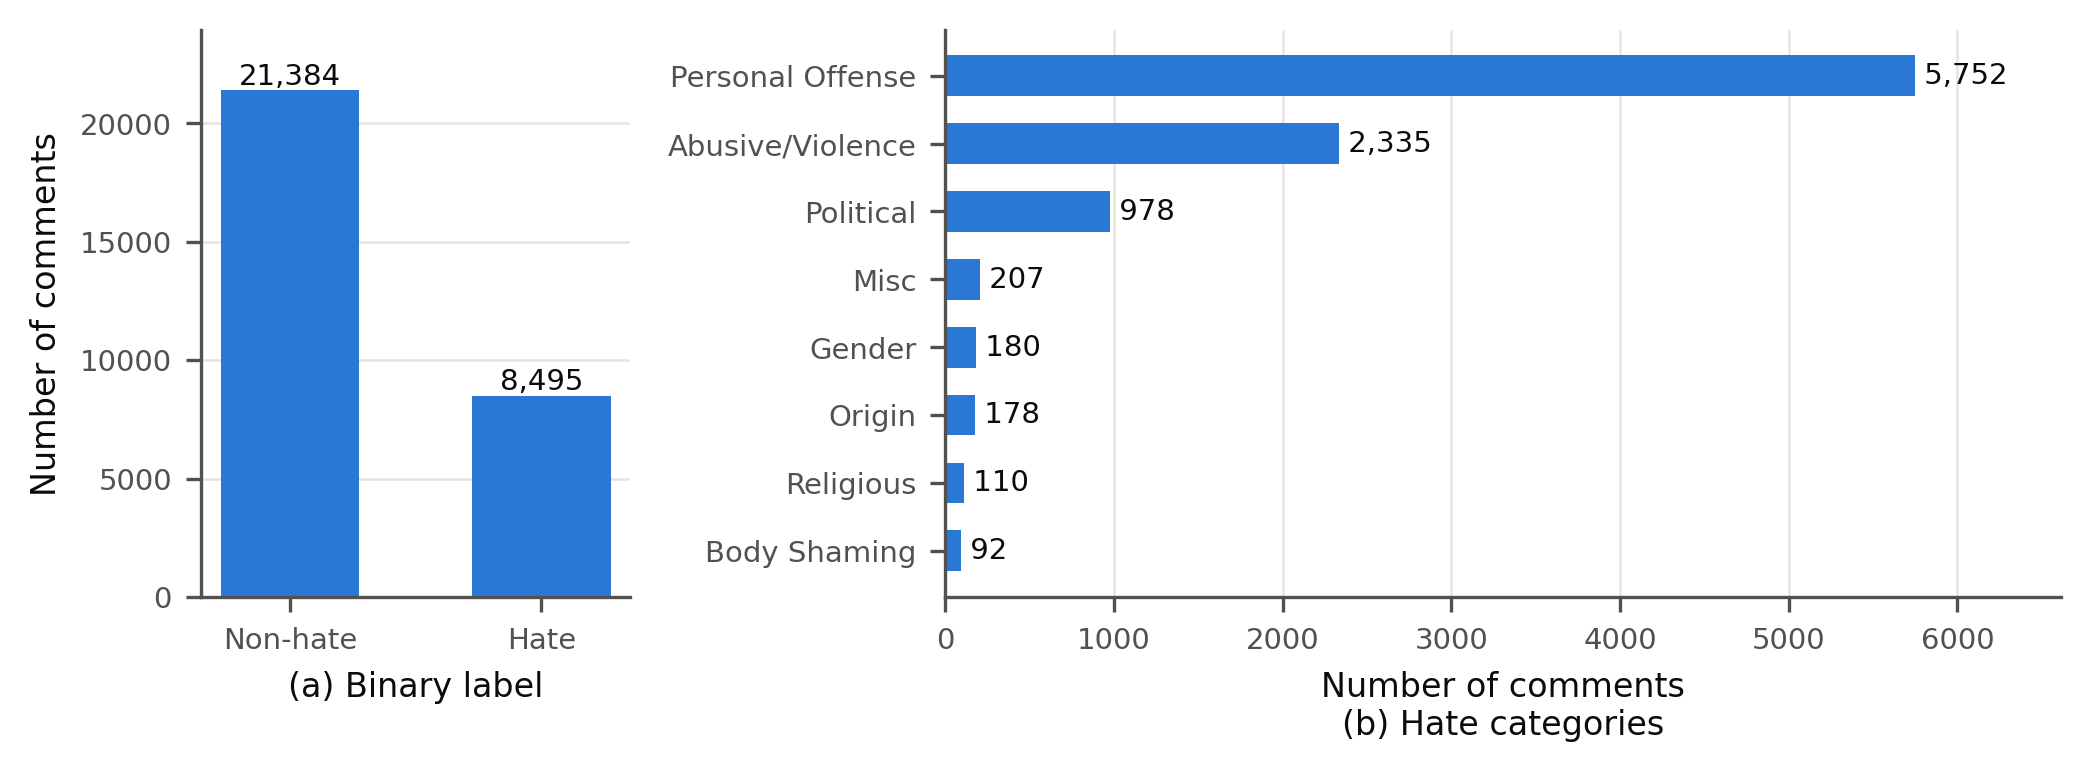
\includegraphics[width=\columnwidth]{figures/fig_02_class_balance.png}
\caption{Class distribution in the training split: (a) binary label, (b) the eight hate categories.}
\label{fig:balance}
\end{figure}

We note one discrepancy. The BanTH paper describes seven categories, whereas the public release contains eight (it adds Misc), and several counts differ; for example, the paper reports \paperBodyShamingTrain{} Body Shaming training comments against \bodyShamingTrain{} in the release, and \paperHateTotal{} hate comments in total against \nHateTotal. The split sizes are identical. The published baselines may therefore have been computed on a slightly different label version.

\subsection{Data Checks and Preprocessing}
We verified that all expected columns are present, that no values are missing, and that all labels are 0 or 1. We found \consistencyViolations{} comments whose binary label contradicts the categories (a non-hate comment with a category or a hate comment without one). Only \testInTrain{} test comment also occurs in the training split, so leakage is negligible. Preprocessing is deliberately light:
\begin{itemize}
\item URLs are removed (\urlRows{} comments) because they carry no linguistic signal.
\item Repeated whitespace and line breaks are collapsed.
\item Spelling variation, emoji, punctuation and letter case are kept: spelling variation is the core difficulty of transliterated text, emoji often carry the tone of a comment, and explanations must refer to the words users actually wrote.
\item No comment is removed, so the split sizes match the official ones.
\end{itemize}
The median comment has \medianWords{} words and 95\% of comments have at most \pNinetyFiveWords{}.

\subsection{Mini Rationale Set}
To evaluate explanations we built a small rationale-annotated subset of the test split. We sampled \ratSample{} hate comments of 3 to 30 words with a fixed seed, using per-category quotas that oversample rare categories. Two team members (Annotators A and B) independently marked, in a spreadsheet, every word that is a reason for the comment being hateful, following the HateXplain principle of marking only the words that justify the label~\cite{mathew2021hatexplain}. The guidelines asked annotators to mark whole insulting phrases, not to mark names unless used as an insult, and to work without seeing each other's sheet. No model or AI suggestions were shown. Annotator A completed \ratA{} comments and Annotator B \ratB; \ratBoth{} comments were annotated by both. Comments left blank were excluded rather than treated as having no rationale. Word-level Cohen's $\kappa$~\cite{cohen1960kappa} on the overlap is \kappaVal{} over \ratWords{} words (raw agreement \rawAgree\%), which corresponds to moderate agreement~\cite{landis1977agreement}.

% ======================================================================
\section{Methodology}

\subsection{Architecture}
Fig.~\ref{fig:arch} shows the system. A comment is tokenised and encoded by XLM-RoBERTa (base, \nParams{}M parameters)~\cite{conneau2020xlmr}. The representation of the first token feeds two linear heads: a binary head with one sigmoid output and a category head with eight sigmoid outputs. Sigmoid outputs allow any number of categories per comment. We chose XLM-R because it was the strongest conventionally fine-tuned encoder in the BanTH benchmark and because its multilingual sub-word vocabulary covers Latin-script Bangla and English. Categories are only reported for comments predicted as hate, mirroring the two-stage setup of BanTH.

\begin{figure}[t]
\centering
\resizebox{\columnwidth}{!}{%
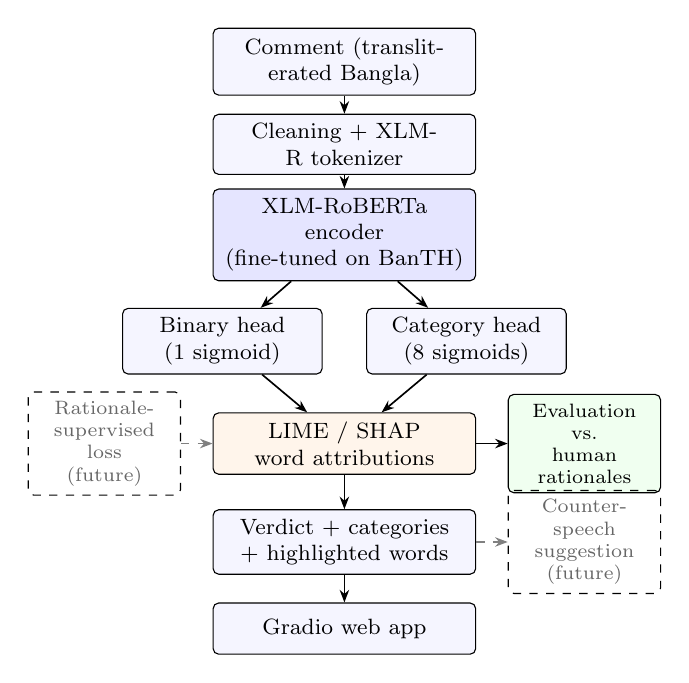
\begin{tikzpicture}[
  box/.style={draw, rounded corners=2pt, align=center, font=\footnotesize, text width=31mm, minimum height=6.5mm, fill=blue!4},
  head/.style={box, text width=23mm},
  side/.style={draw, rounded corners=2pt, align=center, font=\scriptsize, text width=17mm, minimum height=6.5mm},
  fut/.style={side, dashed, text=black!60},
  arr/.style={-{Stealth[length=1.6mm]}, semithick}]
\node[box] (in) at (0, 0) {Comment (transliterated Bangla)};
\node[box] (tok) at (0, -1.05) {Cleaning + XLM-R tokenizer};
\node[box, fill=blue!10] (enc) at (0, -2.2) {XLM-RoBERTa encoder\\(fine-tuned on BanTH)};
\node[head] (bin) at (-1.55, -3.55) {Binary head\\(1 sigmoid)};
\node[head] (cat) at (1.55, -3.55) {Category head\\(8 sigmoids)};
\node[box, fill=orange!8] (xai) at (0, -4.85) {LIME / SHAP\\word attributions};
\node[box] (out) at (0, -6.1) {Verdict + categories\\+ highlighted words};
\node[box] (app) at (0, -7.2) {Gradio web app};
\node[side, fill=green!6, right=4mm of xai] (eval) {Evaluation vs.\\human rationales};
\node[fut, left=4mm of xai] (rs) {Rationale-\\supervised loss\\(future)};
\node[fut, right=4mm of out] (cs) {Counter-speech\\suggestion\\(future)};
\draw[arr] (in) -- (tok);
\draw[arr] (tok) -- (enc);
\draw[arr] (enc) -- (bin);
\draw[arr] (enc) -- (cat);
\draw[arr] (bin) -- (xai);
\draw[arr] (cat) -- (xai);
\draw[arr] (xai) -- (out);
\draw[arr] (out) -- (app);
\draw[arr] (xai) -- (eval);
\draw[arr, dashed, black!50] (rs) -- (xai);
\draw[arr, dashed, black!50] (out) -- (cs);
\end{tikzpicture}}
\caption{System architecture. Dashed boxes are planned extensions that were not implemented.}
\label{fig:arch}
\end{figure}

\subsection{Training}
Both heads use binary cross-entropy, and the total loss is their sum:
\begin{equation}
\mathcal{L} = \mathrm{BCE}(\hat{y}_{b}, y_{b}) + \frac{1}{8}\sum_{c=1}^{8} \mathrm{BCE}_{w_c}(\hat{y}_{c}, y_{c}),
\end{equation}
where $w_c = \sqrt{N^{-}_c / N^{+}_c}$ up-weights positive examples of category $c$ ($N^{+}_c$ and $N^{-}_c$ are its positive and negative training counts). The square root limits the effect of the rarest categories. We follow the BanTH fine-tuning setup where possible (learning rate $2\times10^{-5}$, batch size 32, up to five epochs, early stopping on validation loss). The maximum sequence length is \maxLen{} tokens, which covers 99\% of training comments (\truncPct\% are truncated). Decision thresholds for the binary output and for each category are tuned on the validation split by maximising F1; the test split is never used for tuning. Table~\ref{tab:setup} lists the full setup. We used Hugging Face Transformers~\cite{wolf2020transformers}, PyTorch~\cite{paszke2019pytorch} and scikit-learn~\cite{pedregosa2011sklearn}.

\begin{table}[t]
\caption{Training Setup}
\label{tab:setup}
\centering
\small
\begin{tabular}{lp{5.2cm}}
\toprule
Setting & Value \\
\midrule
Pre-trained encoder & xlm-roberta-base \\
Parameters & 278.1M \\
Loss & BCE (binary) + BCE with pos. weight sqrt(neg/pos) (categories) \\
Optimizer & AdamW, lr 2e-05, weight decay 0.01 \\
LR schedule & linear warm-up (10\%) then linear decay \\
Batch size & 32 \\
Max sequence length & 128 tokens \\
Epochs & max 5, early stopping patience 2 (val. loss); best epoch 4 \\
Dropout & 0.1 \\
Gradient clipping & 1.0 \\
Precision & mixed (fp16) \\
Decision thresholds & tuned on validation (binary 0.58) \\
Random seed & 42 \\
Hardware & Google Colab, Tesla T4 \\
Training time & 18.4 min \\
\bottomrule
\end{tabular}

\end{table}

\subsection{Explanation Methods}
Both methods explain the predicted probability of hate at word level, where a word is a whitespace-separated token; this is the same unit the annotators marked.
\textbf{LIME}~\cite{ribeiro2016lime} removes random subsets of words (1,000 samples per comment) and fits a local linear model to the resulting probabilities.
\textbf{SHAP}~\cite{lundberg2017shap} uses the partition explainer (500 evaluations) to attribute the prediction to words based on Shapley values, with masked words removed as in LIME. Positive scores push towards hate.

\subsection{Evaluation Metrics}
\textbf{Classification.} We report the metrics of the BanTH benchmark~\cite{haider2025banth}: binary macro-F1 and macro-accuracy (the mean of per-class accuracy), and for the categories macro-F1 over the eight labels, subset accuracy (the full label set must be correct) and Hamming loss (the fraction of wrong labels). Because BanTH does not state on which comments its multi-label scores are computed, we report them both on all test comments and on hate comments only.

\textbf{Plausibility.} Following HateXplain~\cite{mathew2021hatexplain}, we compare word scores with human rationales using AUPRC; token F1, where the top-$k$ words are taken with $k$ equal to the number of human-marked words; and IOU F1, the share of comments where the intersection over union of predicted and human rationales is at least 0.5.

\textbf{Faithfulness.} Following ERASER~\cite{deyoung2020eraser}, for a comment $x$ with rationale $r$ and hate probability $p(\cdot)$,
\begin{align}
\text{Comprehensiveness} &= p(x) - p(x \setminus r), \\
\text{Sufficiency} &= p(x) - p(r).
\end{align}
High comprehensiveness means that the rationale was needed, and low sufficiency means that it is enough on its own. We compute both with $k$ equal to the human rationale length, which also allows testing the human rationales, and as AOPC over the top 10, 20, 30 and 50\% of words. A random word ranking serves as a baseline.

\subsection{Keyword-Bias Test and Mitigation}
To test whether the model reacts to individual words rather than meaning, we used \biasNA{} harmless everyday Banglish sentences that contain a word often used in insults or about targeted groups (for example \emph{kukur}, dog; \emph{pagol}, crazy; \emph{hindu}; \emph{awami}) and \biasNB{} harmless sentences without such words. The sentences were checked by the team as natural and non-hateful, so every hate prediction is a false positive. We compare false positive rates (FPR) and use SHAP to check whether the risky word is the main reason.

As a mitigation, we retrained the model with oversampling: words that occur in at least \ifdebias\debMinCount\else 20\fi{} training comments with a hate rate of at least \ifdebias\debMinRate\else 60\fi\% were selected from the training data alone, and every non-hate training comment containing one of them was repeated three extra times. All other settings were unchanged. The probe sentences were not used for training or word selection.

% ======================================================================
\section{Experimental Results and Discussion}

\subsection{Classification}
Table~\ref{tab:comparison} compares our model with the published BanTH results. Our binary macro-F1 of \binF\% is \gapBin{} points below the XLM-R baseline (\blXlmrBin\%) and below the best published model, \blBestBinModel{} (\blBestBin\%), which was further pre-trained on transliterated text. On hate comments, our category macro-F1 of \mlFhate\% is \gapMl{} points below the published XLM-R (\blXlmrMl\%). We therefore consider the model on par with the published fine-tuned encoders, not better. Few-shot GPT-4o obtains the highest category macro-F1 (\blBestMl\%) but a much lower binary score.

\begin{table}[t]
\caption{Test Results Compared With Published BanTH Baselines (\%)}
\label{tab:comparison}
\centering
\small
\resizebox{\columnwidth}{!}{\begin{tabular}{lrrrrr}
\toprule
Model & Bin. F1 & Bin. Acc. & ML F1 & Subset & Hamm.$\downarrow$ \\
\midrule
BanglaBERT & 76.50 & 81.04 & 20.82 & 54.08 & 7.26 \\
mBERT & 74.97 & 80.37 & 28.24 & 52.19 & 7.78 \\
XLM-R & 77.35 & 81.37 & 29.29 & 53.28 & 7.23 \\
TB-BERT & 76.27 & 79.25 & 30.17 & 54.19 & 7.18 \\
TB-mBERT & 77.36 & 82.57 & 27.07 & 54.71 & 7.28 \\
GPT 4o & 70.05 & 74.30 & 36.07 & 22.60 & 16.91 \\
GPT 4o + Few-shot & 68.77 & 74.18 & 39.53 & 26.76 & 14.16 \\
\midrule
Ours, ML on all & 76.23 & 75.99 & 19.53 & 72.37 & 4.34 \\
Ours, ML on hate & 76.23 & 75.99 & 28.89 & 31.45 & 11.03 \\
\bottomrule
\end{tabular}
}
\\[2pt]
\footnotesize Baseline values from~\cite{haider2025banth}. ML: multi-label; ``on all'' and ``on hate'' give the comments the multi-label scores are computed on.
\end{table}

Two differences affect this comparison. First, our macro-accuracy (\binMacroAcc\%) is lower than our plain accuracy (\binAcc\%), whereas the published macro-accuracy values are close to our plain accuracy; we follow the definition stated in the BanTH paper and report both. Second, our subset accuracy and Hamming loss depend strongly on which comments are scored (Table~\ref{tab:comparison}), and the published values lie between our two settings. Together with the label-version difference noted in Section~\ref{sec:dataset}, this means that small gaps should not be over-interpreted.

Table~\ref{tab:binary} gives the binary results at the default threshold of 0.5 and at the validation-tuned threshold (\binThr). Fig.~\ref{fig:confusion} shows that \pctFN\% of hate comments are missed and \pctFP\% of non-hate comments are wrongly flagged. Training took \trainMinutes{} minutes on a Colab T4 GPU; the validation loss was lowest at epoch \bestEpoch{}.

\begin{table}[t]
\caption{Binary Results on the Test Split (\%)}
\label{tab:binary}
\centering
\small
\resizebox{\columnwidth}{!}{\begin{tabular}{lrrrrrr}
\toprule
Threshold & M-F1 & M-Acc. & Acc. & P & R & F1 \\
\midrule
0.5 & 75.50 & 76.20 & 79.54 & 62.89 & 68.46 & 65.55 \\
Tuned (val.) & 76.23 & 75.99 & 80.83 & 66.80 & 64.78 & 65.77 \\
\bottomrule
\end{tabular}
}
\end{table}

\begin{figure}[t]
\centering
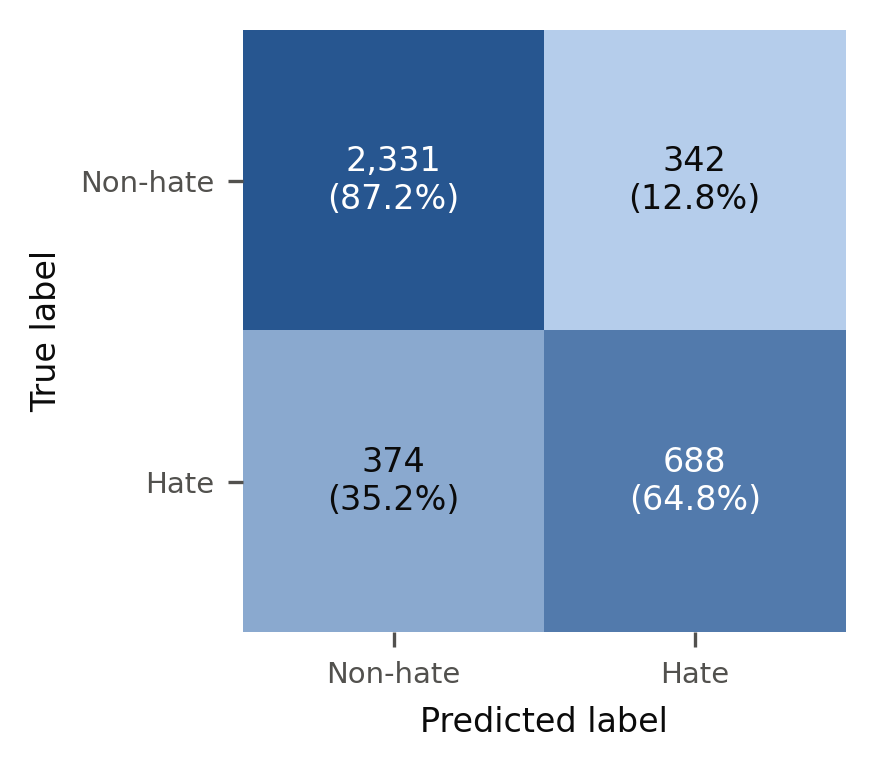
\includegraphics[width=0.72\columnwidth]{figures/fig_05_confusion_matrix.png}
\caption{Binary confusion matrix on the test split (tuned threshold). Percentages are relative to the true class.}
\label{fig:confusion}
\end{figure}

\subsection{Per-Category Results}
Table~\ref{tab:percat} and Fig.~\ref{fig:percat} show a clear dependence on category size. Personal Offense (F1 \catPO\%), Abusive/Violence (\catAV\%) and Political (\catPol\%) are learned reasonably, whereas Religious, Origin and Body Shaming reach an F1 of zero on all test comments. These categories have 14 to 23 test comments, so their thresholds, tuned on a similarly small validation set, do not transfer to the test split, and single errors change their scores considerably.

\begin{table}[t]
\caption{Per-Category Test Results (\%)}
\label{tab:percat}
\centering
\small
\resizebox{\columnwidth}{!}{\begin{tabular}{lrrrrrr}
\toprule
Category & Train & Test & P & R & F1 & F1\textsubscript{hate} \\
\midrule
Political & 978 & 117 & 38.6 & 33.3 & 35.8 & 50.7 \\
Religious & 110 & 18 & 0.0 & 0.0 & 0.0 & 19.0 \\
Gender & 180 & 23 & 8.6 & 13.0 & 10.3 & 23.5 \\
Personal Offense & 5{,}752 & 715 & 51.5 & 62.0 & 56.2 & 67.1 \\
Abusive/Violence & 2{,}335 & 304 & 50.8 & 43.1 & 46.6 & 50.1 \\
Origin & 178 & 23 & 0.0 & 0.0 & 0.0 & 0.0 \\
Body Shaming & 92 & 14 & 0.0 & 0.0 & 0.0 & 12.5 \\
Misc & 207 & 30 & 8.0 & 6.7 & 7.3 & 8.2 \\
\bottomrule
\end{tabular}
}
\\[2pt]
\footnotesize F1: all test comments; F1\textsubscript{hate}: hate comments only.
\end{table}

\begin{figure}[t]
\centering
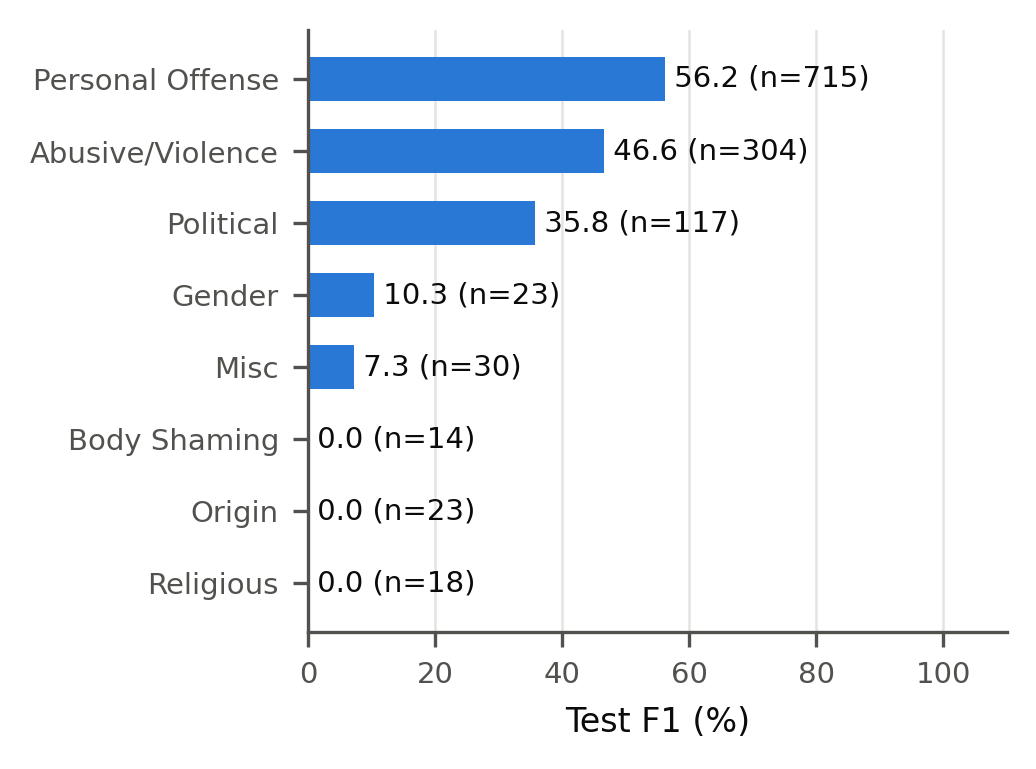
\includegraphics[width=0.85\columnwidth]{figures/fig_06_per_category_f1.png}
\caption{Test F1 per category. The number of test comments per category is given in brackets.}
\label{fig:percat}
\end{figure}

\subsection{Plausibility}
Table~\ref{tab:plaus} shows that both methods agree with human rationales far better than the random baseline. Against Annotator A (\plNA{} comments), SHAP reaches a token F1 of \tokFShapA{} and LIME \tokFLimeA, against \tokFRandomA{} for random scores; the ranking is the same against Annotator B. The two methods also largely agree with each other: on a separate set of eight test comments selected by a fixed rule, they share on average \topThreeOverlap{} of their top-three words. Fig.~\ref{fig:human} shows one comment on which both annotators and both methods mark nearly the same words.

\begin{table}[t]
\caption{Plausibility Against Human Rationales}
\label{tab:plaus}
\centering
\small
\begin{tabular}{cclrrr}
\toprule
Ref. & $n$ & Method & AUPRC & Tok. F1 & IOU F1 \\
\midrule
A & 91 & LIME & 0.805 & 0.683 & 0.527 \\
A & 91 & SHAP & 0.808 & 0.715 & 0.604 \\
A & 91 & Random & 0.627 & 0.518 & 0.352 \\
\midrule
B & 55 & LIME & 0.777 & 0.658 & 0.545 \\
B & 55 & SHAP & 0.777 & 0.690 & 0.600 \\
B & 55 & Random & 0.567 & 0.466 & 0.327 \\
\bottomrule
\end{tabular}

\end{table}

\begin{figure*}[t]
\centering
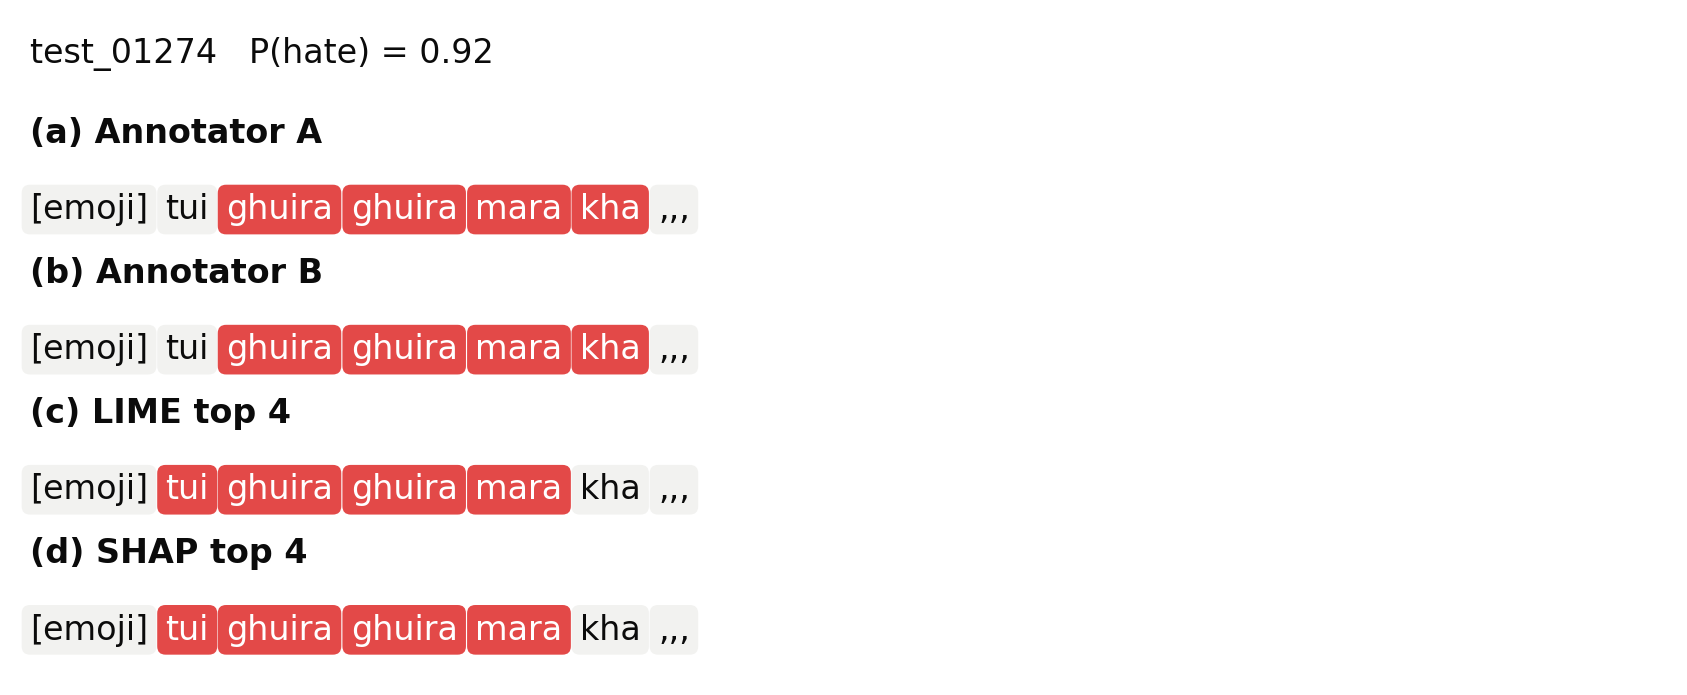
\includegraphics[width=0.8\textwidth]{figures/fig_08_human_vs_model_test_01274.png}
\caption{Words marked by the two annotators (a, b) and the top words selected by LIME (c) and SHAP (d) for one test comment. Both methods rank the informal pronoun \emph{tui} (``you'') above \emph{kha}, which the annotators marked.}
\label{fig:human}
\end{figure*}

\subsection{Faithfulness}
Table~\ref{tab:faith} shows that the explanations are faithful to the model. Deleting the top SHAP words lowers the hate probability by \compShap{} on average, and the top LIME words by \compLime, compared with \compRandom{} for random words. Keeping only the top words even raises the probability (negative sufficiency). This differs from the HateBRXplain finding that plausible explanations were not faithful~\cite{salles2025hatebrxplain}; one possible explanation is that hate in BanTH is often carried by explicit insult words. The human rationales are also comprehensive (\compHuman), which indicates that the model largely relies on the words that people consider hateful.

\begin{table}[t]
\caption{Faithfulness on \faithN{} Annotated Test Comments}
\label{tab:faith}
\centering
\small
\resizebox{\columnwidth}{!}{\begin{tabular}{lrrrr}
\toprule
Rationale & Comp.$\uparrow$ & Suff.$\downarrow$ & Comp.\textsubscript{AOPC}$\uparrow$ & Suff.\textsubscript{AOPC}$\downarrow$ \\
\midrule
Human & 0.41 & -0.02 & -- & -- \\
LIME & 0.47 & -0.13 & 0.41 & -0.12 \\
SHAP & 0.48 & -0.13 & 0.42 & -0.13 \\
Random & 0.16 & 0.18 & 0.08 & 0.27 \\
\bottomrule
\end{tabular}
}
\end{table}

\subsection{Error Analysis}
The explanations point to a recurring error. In the comment of Fig.~\ref{fig:human}, both methods rank the informal pronoun \emph{tui} highly, and in a non-hate test comment that the model flagged, both LIME and SHAP blame \emph{Tor}/\emph{Tore}, other forms of the same pronoun. These pronouns are frequent in insults but are also used between friends. Missed hate comments, by contrast, often contain mild or context-dependent insults whose probability stays just below the threshold. These observations motivated the keyword-bias test.

\subsection{Keyword Bias}
\label{sec:bias}
Table~\ref{tab:bias} and Fig.~\ref{fig:bias} confirm the pattern. \biasFlagA{} of \biasNA{} harmless sentences with a risky word (\biasFprA\%) were flagged as hate, against \biasFlagB{} of \biasNB{} (\biasFprB\%) without one, and SHAP named the risky word as the top reason in \biasShapTop\% of the first group. The training data explain why: comments containing \emph{kuttar} are hate in \hrKuttar\% of cases, \emph{kukur} in \hrKukur\% and \emph{baccha} in \hrBaccha\%, against \trainHatePct\% overall. Group terms such as \emph{hindu} (\hrHindu\%) and \emph{bnp} (\hrBnp\%) are not strongly tied to hate in the data, and harmless sentences with them were not flagged. The bias therefore concerns insult-associated vocabulary rather than mentions of religious or political groups.

\begin{table}[t]
\caption{Keyword-Bias Test on Harmless Sentences}
\label{tab:bias}
\centering
\small
\resizebox{\columnwidth}{!}{\begin{tabular}{lrrrrr}
\toprule
Group & $n$ & Flagged & FPR (\%) & Mean $p$ & SHAP top (\%) \\
\midrule
A: with risky word & 69 & 18 & 26.1 & 0.33 & 55.1 \\
B: without risky word & 31 & 1 & 3.2 & 0.12 & -- \\
\bottomrule
\end{tabular}
}
\\[2pt]
\footnotesize All sentences are non-hateful, so every flagged sentence is a false positive.
\end{table}

\begin{figure}[t]
\centering
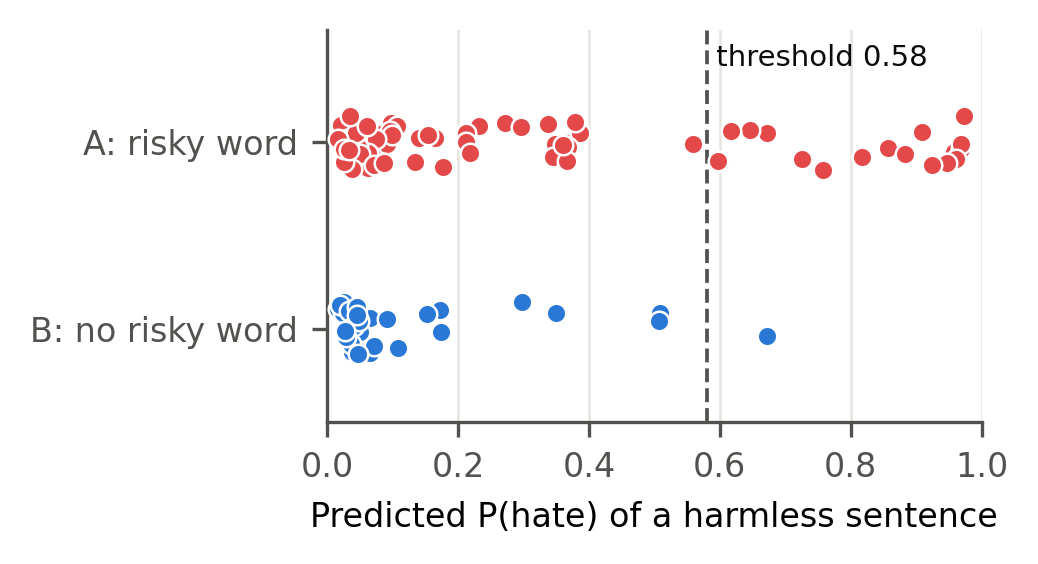
\includegraphics[width=0.9\columnwidth]{figures/fig_10_keyword_bias.png}
\caption{Predicted hate probability of harmless sentences with (A) and without (B) insult-associated words. Points right of the dashed threshold are false positives.}
\label{fig:bias}
\end{figure}

\subsection{Bias Mitigation}
\ifdebias
Table~\ref{tab:debias} and Fig.~\ref{fig:debias} compare the main model with the model trained with oversampling. The word rule selected \debNWords{} words, and \debNRepeated{} non-hate training comments were repeated, giving \debTrainRows{} training rows. On real non-hate test comments that contain one of these words (\debTestNWith{} comments), the false positive rate fell from \debTestOldWith\% to \debTestNewWith\%, while it stayed practically unchanged for the other \debTestNWithout{} non-hate comments (\debTestOldWithout\% and \debTestNewWithout\%). On the harmless probe sentences, it fell from \biasFprA\% to \debFprA\% with a risky word and from \biasFprB\% to \debFprB\% without one.

The fix is not free. Binary macro-F1 dropped by \debBinDrop{} points to \debBinF\%, and category macro-F1 on hate comments dropped by \debMlDrop{} points to \debMlF\%. The validation loss was lowest at epoch \debBestEpoch{}, so the category head was trained for fewer epochs than in the main model, which may explain part of this drop. We therefore keep the main model as our primary result and report the oversampled model as evidence that the bias can be reduced with existing data, at a cost that future work should address, for example with rationale-supervised training~\cite{mathew2021hatexplain}.

\begin{table}[t]
\caption{Effect of Oversampling on Accuracy and False Positive Rates (\%)}
\label{tab:debias}
\centering
\small
\resizebox{\columnwidth}{!}{\begin{tabular}{lrrrrrr}
\toprule
Model & Bin. F1 & ML F1 & Probe A & Probe B & Test w/ & Test w/o \\
\midrule
Main model & 76.23 & 28.89 & 26.1 & 3.2 & 74.8 & 9.1 \\
With oversampling & 75.46 & 22.05 & 18.8 & 0.0 & 33.8 & 9.2 \\
\bottomrule
\end{tabular}
}
\\[2pt]
\footnotesize ML F1 on hate comments. Probe A/B: harmless sentences with/without a risky word. Test w/, w/o: non-hate test comments with/without a listed word.
\end{table}

\begin{figure}[t]
\centering
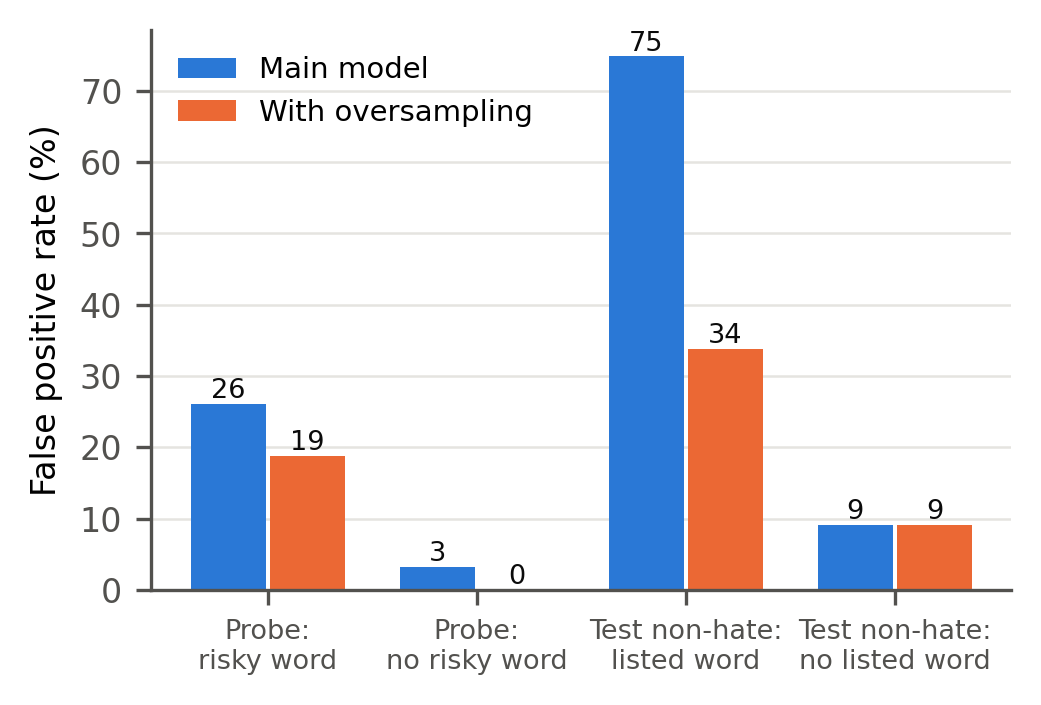
\includegraphics[width=0.9\columnwidth]{figures/fig_11_debias_fpr.png}
\caption{False positive rates of the main model and the model trained with oversampling.}
\label{fig:debias}
\end{figure}
\else
Results of the mitigation experiment are pending.
\fi

% ======================================================================
\section{Demo System}
We deployed the model as a Gradio~\cite{abid2019gradio} web application that runs from Google Colab with a public link (Fig.~\ref{fig:demo}). A user enters a comment or selects an example; the application shows the verdict with its probability and decision threshold, the SHAP or LIME word highlights, and the eight category scores with the detected categories marked. Explanations are computed on demand within a few seconds on a T4 GPU. A separate list of harmless sentences from the keyword-bias test shows the known weakness, and an information panel reports the main evaluation results, read from the saved result files. The intended users are content moderators and monitoring organisations: the highlights let them check a flag quickly instead of trusting the label. The application is a research prototype meant to assist human decisions, not to remove content automatically.

\begin{figure}[t]
\centering
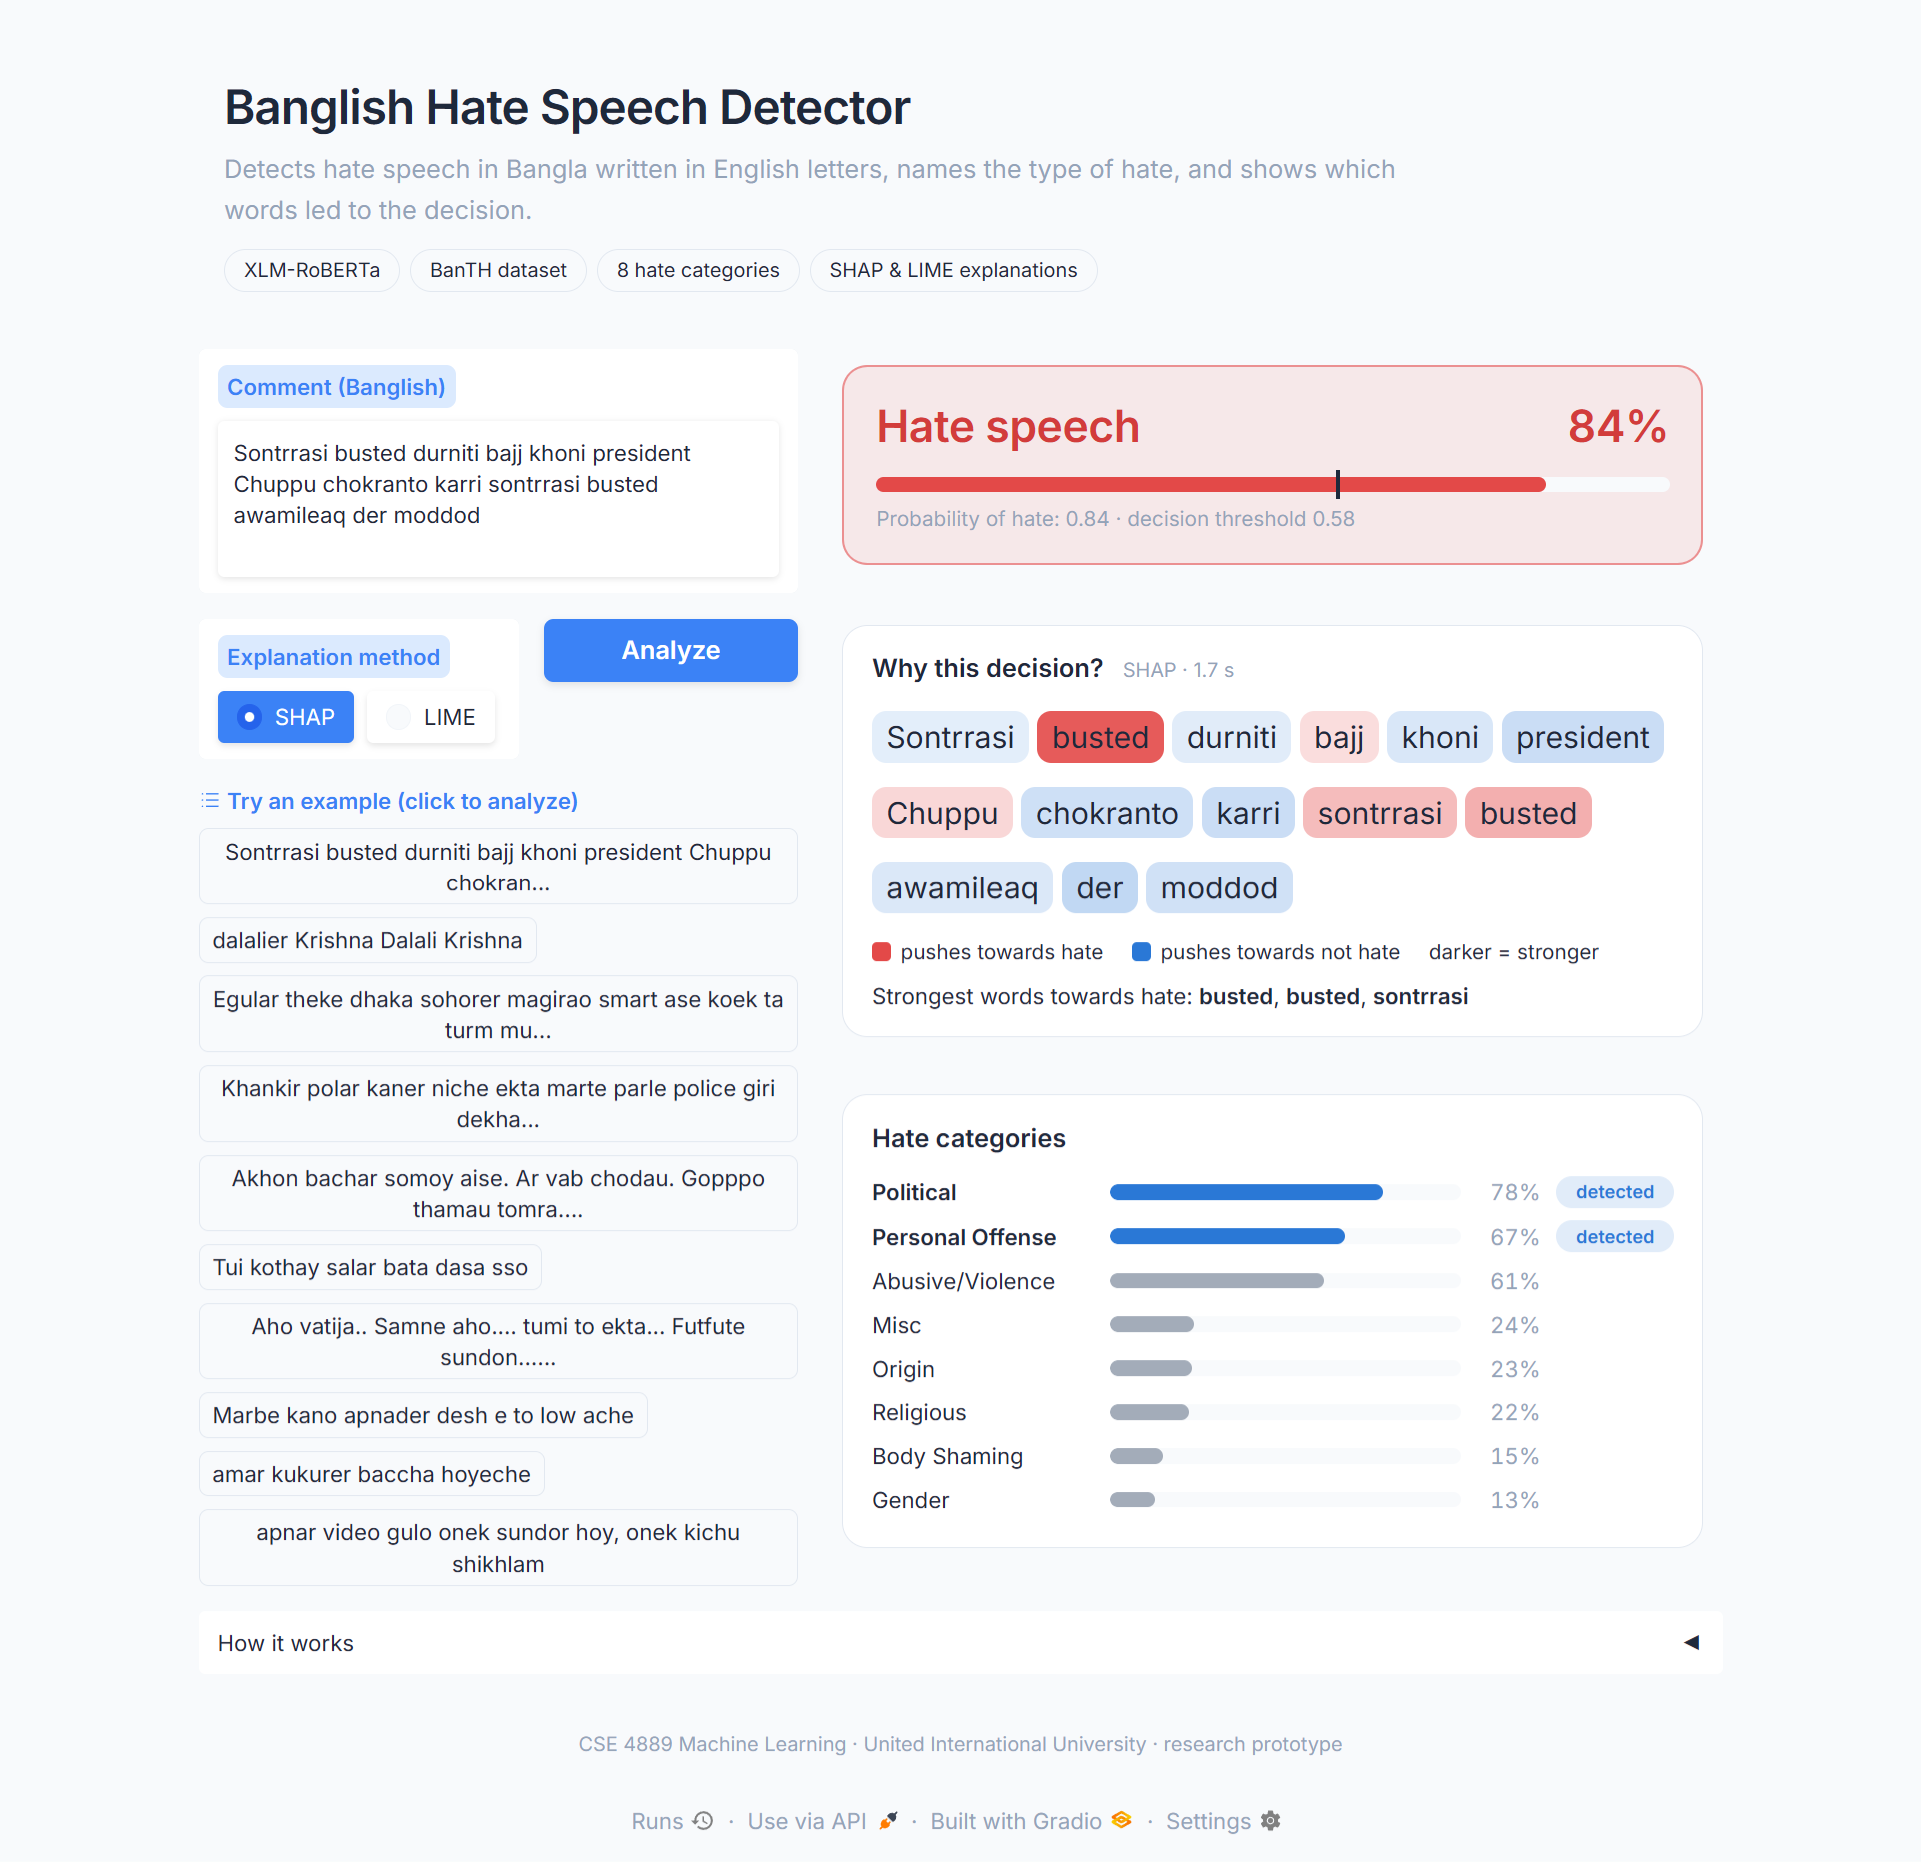
\includegraphics[width=\columnwidth]{figures/fig_09_demo_hate.png}
\caption{The web application analysing a hate comment: verdict, SHAP word attributions and category scores.}
\label{fig:demo}
\end{figure}

% ======================================================================
\section{Limitations and Future Work}
\textbf{Limitations.} The rationale set is small (\ratSample{} comments, two annotators, \ratBoth{} annotated by both), and agreement is moderate ($\kappa$ = \kappaVal); the main plausibility reference is a single annotator. Rare categories are not learned reliably, and their test scores rest on 14 to 23 comments. The published baselines may use a different label version than the public release. The keyword-bias test uses \biasNA{} + \biasNB{} sentences and shows a pattern rather than a precise rate. The mitigation model stopped early at epoch \debBestEpoch{}, so its lower category scores may partly reflect shorter training rather than the oversampling itself. Emoji cannot be shown in our figures, although they are part of the model input.

\textbf{Future work.} The following items were planned but deliberately deferred: (i) rationale-supervised training with an auxiliary loss that aligns attributions with human rationales, which HateXplain found to reduce bias~\cite{mathew2021hatexplain}; (ii) data augmentation for rare categories; (iii) a counter-speech module that drafts a de-escalating reply for moderators; (iv) a larger rationale set with more annotators and a full fairness audit across target communities; and (v) attention-based explanations. We also plan to test encoders further pre-trained on transliterated Bangla, which performed best in the BanTH benchmark.

\textbf{Ethics.} BanTH consists of public YouTube comments; we show offensive examples only to illustrate the task and do not publish user identities. Annotating hateful content can be distressing, so the guidelines included a content warning and encouraged breaks. False positives on harmless everyday language, as found in Section~\ref{sec:bias}, could silence ordinary users if such a model were used without human review.

% ======================================================================
\section{Conclusion}
We presented an explainable multi-label hate speech detector for transliterated Bangla. The dual-head XLM-R model performs on par with published fine-tuned baselines on BanTH (binary macro-F1 \binF\%). Evaluated against human rationales, SHAP and LIME explanations are clearly more plausible than random and faithful to the model. The same explanations exposed a keyword bias: harmless sentences containing insult-associated words are flagged far more often than other harmless sentences. Oversampling harmless training comments with such words reduced this bias substantially but lowered category performance, so reducing the bias without losing accuracy remains open. The rationale set, the bias test and the web application provide a starting point for trustworthy moderation tools for transliterated Bangla.

\bibliographystyle{IEEEtran}
\bibliography{references}

\end{document}
